% Options for packages loaded elsewhere
% Options for packages loaded elsewhere
\PassOptionsToPackage{unicode}{hyperref}
\PassOptionsToPackage{hyphens}{url}
%
\documentclass[
  ignorenonframetext,
]{beamer}
\newif\ifbibliography
\usepackage{pgfpages}
\setbeamertemplate{caption}[numbered]
\setbeamertemplate{caption label separator}{: }
\setbeamercolor{caption name}{fg=normal text.fg}
\beamertemplatenavigationsymbolsempty
% remove section numbering
\setbeamertemplate{part page}{
  \centering
  \begin{beamercolorbox}[sep=16pt,center]{part title}
    \usebeamerfont{part title}\insertpart\par
  \end{beamercolorbox}
}
\setbeamertemplate{section page}{
  \centering
  \begin{beamercolorbox}[sep=12pt,center]{section title}
    \usebeamerfont{section title}\insertsection\par
  \end{beamercolorbox}
}
\setbeamertemplate{subsection page}{
  \centering
  \begin{beamercolorbox}[sep=8pt,center]{subsection title}
    \usebeamerfont{subsection title}\insertsubsection\par
  \end{beamercolorbox}
}
% Prevent slide breaks in the middle of a paragraph
\widowpenalties 1 10000
\raggedbottom
\AtBeginPart{
  \frame{\partpage}
}
\AtBeginSection{
  \ifbibliography
  \else
    \frame{\sectionpage}
  \fi
}
\AtBeginSubsection{
  \frame{\subsectionpage}
}
\usepackage{iftex}
\ifPDFTeX
  \usepackage[T1]{fontenc}
  \usepackage[utf8]{inputenc}
  \usepackage{textcomp} % provide euro and other symbols
\else % if luatex or xetex
  \usepackage{unicode-math} % this also loads fontspec
  \defaultfontfeatures{Scale=MatchLowercase}
  \defaultfontfeatures[\rmfamily]{Ligatures=TeX,Scale=1}
\fi
\usepackage{lmodern}

\usetheme[]{metropolis}
\ifPDFTeX\else
  % xetex/luatex font selection
\fi
% Use upquote if available, for straight quotes in verbatim environments
\IfFileExists{upquote.sty}{\usepackage{upquote}}{}
\IfFileExists{microtype.sty}{% use microtype if available
  \usepackage[]{microtype}
  \UseMicrotypeSet[protrusion]{basicmath} % disable protrusion for tt fonts
}{}
\makeatletter
\@ifundefined{KOMAClassName}{% if non-KOMA class
  \IfFileExists{parskip.sty}{%
    \usepackage{parskip}
  }{% else
    \setlength{\parindent}{0pt}
    \setlength{\parskip}{6pt plus 2pt minus 1pt}}
}{% if KOMA class
  \KOMAoptions{parskip=half}}
\makeatother


\usepackage{longtable,booktabs,array}
\usepackage{calc} % for calculating minipage widths
\usepackage{caption}
% Make caption package work with longtable
\makeatletter
\def\fnum@table{\tablename~\thetable}
\makeatother
\usepackage{graphicx}
\makeatletter
\newsavebox\pandoc@box
\newcommand*\pandocbounded[1]{% scales image to fit in text height/width
  \sbox\pandoc@box{#1}%
  \Gscale@div\@tempa{\textheight}{\dimexpr\ht\pandoc@box+\dp\pandoc@box\relax}%
  \Gscale@div\@tempb{\linewidth}{\wd\pandoc@box}%
  \ifdim\@tempb\p@<\@tempa\p@\let\@tempa\@tempb\fi% select the smaller of both
  \ifdim\@tempa\p@<\p@\scalebox{\@tempa}{\usebox\pandoc@box}%
  \else\usebox{\pandoc@box}%
  \fi%
}
% Set default figure placement to htbp
\def\fps@figure{htbp}
\makeatother

\ifLuaTeX
  \usepackage{luacolor}
  \usepackage[soul]{lua-ul}
\else
  \usepackage{soul}
  \makeatletter
  \let\HL\hl
  \renewcommand\hl{% fix for beamer highlighting
    \let\set@color\beamerorig@set@color
    \let\reset@color\beamerorig@reset@color
    \HL}
  \makeatother
\fi




\setlength{\emergencystretch}{3em} % prevent overfull lines

\providecommand{\tightlist}{%
  \setlength{\itemsep}{0pt}\setlength{\parskip}{0pt}}



 


\setbeamerfont{title}{size=\large} \usepackage{hyperref} \setbeamertemplate{footline}[frame number]
\makeatletter
\@ifpackageloaded{caption}{}{\usepackage{caption}}
\AtBeginDocument{%
\ifdefined\contentsname
  \renewcommand*\contentsname{Table of contents}
\else
  \newcommand\contentsname{Table of contents}
\fi
\ifdefined\listfigurename
  \renewcommand*\listfigurename{List of Figures}
\else
  \newcommand\listfigurename{List of Figures}
\fi
\ifdefined\listtablename
  \renewcommand*\listtablename{List of Tables}
\else
  \newcommand\listtablename{List of Tables}
\fi
\ifdefined\figurename
  \renewcommand*\figurename{Figure}
\else
  \newcommand\figurename{Figure}
\fi
\ifdefined\tablename
  \renewcommand*\tablename{Table}
\else
  \newcommand\tablename{Table}
\fi
}
\@ifpackageloaded{float}{}{\usepackage{float}}
\floatstyle{ruled}
\@ifundefined{c@chapter}{\newfloat{codelisting}{h}{lop}}{\newfloat{codelisting}{h}{lop}[chapter]}
\floatname{codelisting}{Listing}
\newcommand*\listoflistings{\listof{codelisting}{List of Listings}}
\makeatother
\makeatletter
\makeatother
\makeatletter
\@ifpackageloaded{caption}{}{\usepackage{caption}}
\@ifpackageloaded{subcaption}{}{\usepackage{subcaption}}
\makeatother

\usepackage{bookmark}
\IfFileExists{xurl.sty}{\usepackage{xurl}}{} % add URL line breaks if available
\urlstyle{same}
\hypersetup{
  pdfauthor={Giorgio Arcara},
  hidelinks,
  pdfcreator={LaTeX via pandoc}}


\author{Giorgio Arcara}
\date{}

\begin{document}


\begin{frame}
% TITLE SLIDES
\title{Metodi Statistici per la Neuropsicologia Forense\\ \vspace{1em} \emph{Introduzione}}
\author{Giorgio Arcara,\\ Università di Padova \\ IRCCS San Camillo, Venezia}

\titlegraphic{

\vspace*{7cm}

\includegraphics[scale=0.15]{Figures/LogoSanCamilloIRCCS_Unipd_alpha.png}
\begin{center}
\vspace{-2.2em}

\includegraphics[scale=0.15]{Figures/CC_license_3_0.png}
\end{center}
}
\date{\today}
\maketitle
\end{frame}

\begin{frame}{Lezione di oggi}
\phantomsection\label{lezione-di-oggi}
\begin{itemize}
\tightlist
\item
  Presentazione del docente e del corso.
\item
  Aspetti organizzativi del corso.
\item
  Obiettivi formativi e ``spirito'' del corso.
\end{itemize}
\end{frame}

\section{Introduzione}\label{introduzione}

\begin{frame}{CV Giorgio Arcara}
\phantomsection\label{cv-giorgio-arcara}
\footnotesize

\begin{itemize}
\item
  Laurea in Psicologia presso Unipd (2005)
\item
  Master in Neuropsicologia dei disturbi cognitivi acquisiti (2006)
\item
  Vari post-doc presso dipartimenti (psicologia, ingegneria,
  neuroscienze)
\item
  Dal 2016 Ricercatore presso IRCCS San Camillo di Venezia.
\item
  Dal 2025 Professore Associato in Psicometria - Università di Padova.
\end{itemize}

\pause

\hfill
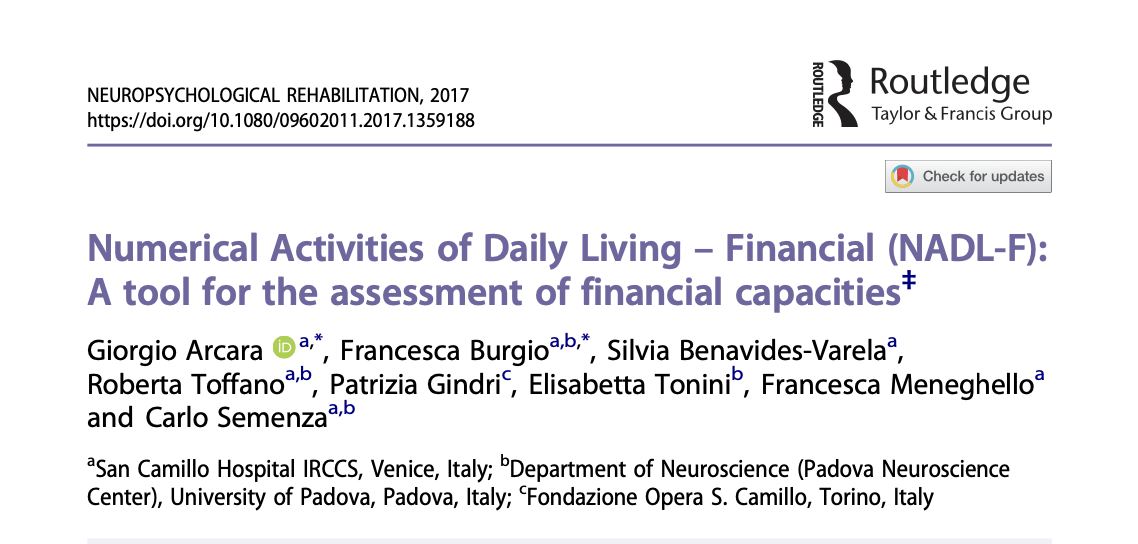
\includegraphics[width=0.6\linewidth,height=\textheight,keepaspectratio]{Figures/NADL_F.png}
\end{frame}

\begin{frame}{Contatti e riferimenti}
\phantomsection\label{contatti-e-riferimenti}
\centering

\href{https://giorgioarcara.github.io}{\ul{https://giorgioarcara.github.io}}

\href{https://www.dpg.unipd.it/category/ruoli/personale-docente?key=4D0707A2DD6FCCD50B90E4C9F316A625}{\ul{pagina
personale unipd}}

\href{mailto:giorgio.arcara@unipd.it}{\nolinkurl{giorgio.arcara@unipd.it}}
\end{frame}

\begin{frame}{Aspetti organizzativi - Lezioni}
\phantomsection\label{aspetti-organizzativi---lezioni}
\begin{itemize}
\tightlist
\item
  Lezioni online principalmente il mercoledì e il giovedì (dalle 9.00
  alle 11.30 circa)
\item
  Le lezioni prevedono didattica frontale (interattiva), esercitazioni
  in classe.
\item
  Saranno trattate poche formule.
\item
  Sono benvenute le domande (in qualsiasi momento).
\item
  Sarà in alcuni casi mostrato del codice in R, ma non è richiesto per
  l'esame.
\end{itemize}
\end{frame}

\begin{frame}{Orari lezioni (dettaglio)}
\phantomsection\label{orari-lezioni-dettaglio}
\scriptsize

\begin{itemize}
\tightlist
\item
  Mercoledì 8 Ottobre: 9.00 - 11.30
\item
  Giovedì 9 Ottobre: 9.00 - 11.30
\item
  Mercoledì 15 Ottobre: 9.00 - 11.30
\item
  Giovedì 16 Ottobre: 9.00 - 11.30
\item
  Mercoledì 22 Ottobre: 9.00 - 11.30
\item
  Giovedì 23 Ottobre: 9.00 - 11.30
\item
  Mercoledì 5 Novembre: 9.00 - 11.30
\item
  Giovedì 6 Novembre: 9.00 - 11.30
\item
  Mercoledì 12 Novembre: 9.00 - 11.30
\item
  Giovedì 13 Novembre: 9.00 - 11.30
\item
  Mercoledì 19 Novembre: 9.00 - 11.30
\item
  Giovedì 20 Novembre: 9.00 - 11.30
\item
  Mercoledì 26 Novembre: 9.00 - 11.30
\item
  Giovedì 27 Novembre: 9.00 - 11.30
\end{itemize}
\end{frame}

\begin{frame}{Aspetti organizzativi - Materiali}
\phantomsection\label{aspetti-organizzativi---materiali}
\textbf{Condividerò tutto il materiale utilizzato e mostrato}

I materiali principali sono le slides e materiali aggiuntivi che vi
saranno forniti durante il corso. I materiali li troverete anche al
link:

\href{\%5Bhttps://github.com/giorgioarcara/stat_forensic_neuropsy}{\ul{https://github.com/giorgioarcara/stat\_forensic\_neuropsy}}

Condividerò anche script di R e sarà dato risalto a ``simulazioni'' di
dati per comprensione dei concetti, con script sviluppati durante il
corso (utili, non necessari).
\end{frame}

\begin{frame}{Aspetti organizzativi - Materiali}
\phantomsection\label{aspetti-organizzativi---materiali-1}
\begin{columns}
\column{0.5\textwidth}
\small
\emph{Mondini, S., Cappelletti, M., \& Arcara, G. (2022). Methodology in Neuropsychological Assessment: An Interpretative Approach to Guide Clinical Practice. Taylor \& Francis.}\\

testo di approfondimento, \textbf{non necessario}.

\column{0.5\textwidth}

\begin{figure}
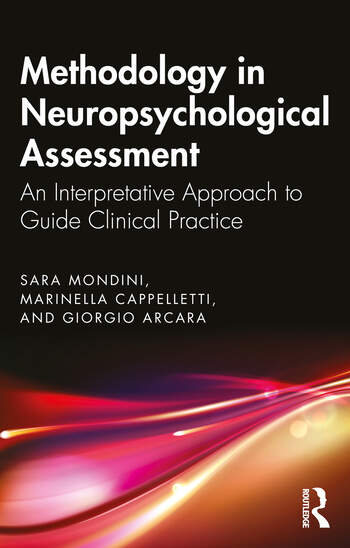
\includegraphics[scale=0.5]{Figures/Methodology_book.png}
\end{figure}

\end{columns}
\end{frame}

\begin{frame}{Aspetti organizzativi - Materiali aggiuntivi}
\phantomsection\label{aspetti-organizzativi---materiali-aggiuntivi}
\begin{itemize}
\item
  Libro gratuito su statistica base ed R
  \href{https://learningstatisticswithr.com/}{\underline{https://learningstatisticswithr.com/}}
\item
  Libro gratuito su psicometria (più avanzato)
  \href{https://personality-project.org/r/book/}{\underline{https://personality-project.org/r/book/}}
\item
  Libro in corso di scrittura
  \href{https://giorgioarcara.github.io/oip-book/}{\underline{https://giorgioarcara.github.io/oip-book/}}
\end{itemize}
\end{frame}

\begin{frame}{Aspetti organizzativi - Esami}
\phantomsection\label{aspetti-organizzativi---esami}
Gli esami saranno scritti con:

\begin{itemize}
\tightlist
\item
  domande aperte su aspetti teorici.
\item
  domande su scenari applicativi in cui ragionare per applicare le
  conoscenze sviluppate.
\end{itemize}

Gli esami saranno poco nozionistici e più di ragionamento

\underline{Non sarà necessario ricordare a memoria nessuna formula}
\end{frame}

\begin{frame}{Obiettivi del corso}
\phantomsection\label{obiettivi-del-corso}
Partiamo dalla fine:

\begin{itemize}
\tightlist
\item
  Fornire elementi di conoscenza statistica e ragionamento critico utili
  per la neuropsicologia forense
\item
  Fornire conoscenze sia per la pratica di psicologia forense, sia per
  chi vuole fare ricerca in ambito forense.
\item
  Fornire conoscenze sull'elemento cardine per la valutazione forense:
  il test cognitivo o neuropsicologico, con le sue potenzialità e
  limiti.
\end{itemize}

\emph{Obiettivo bonus}: superare alcuni traumi che vi ha dato la
statistica a Psicologia
\end{frame}

\begin{frame}{Perché è utile la statistica per il neuropsicologo
forense?}
\phantomsection\label{perchuxe9-uxe8-utile-la-statistica-per-il-neuropsicologo-forense}
\begin{columns}
\column{0.5\textwidth}

\begin{figure}
\includegraphics[width=0.8\textwidth]{Figures/Motore.png}
\end{figure}
\tiny{Non serve conoscere come funziona un motore per guidare una macchina. Basta sapere cosa è giusto o sbagliato fare con pedali, cambio e volante. (Aforisma approssimativo di H. R. Baayen, 2008 circa)}


\column{0.5\textwidth}

\begin{figure}
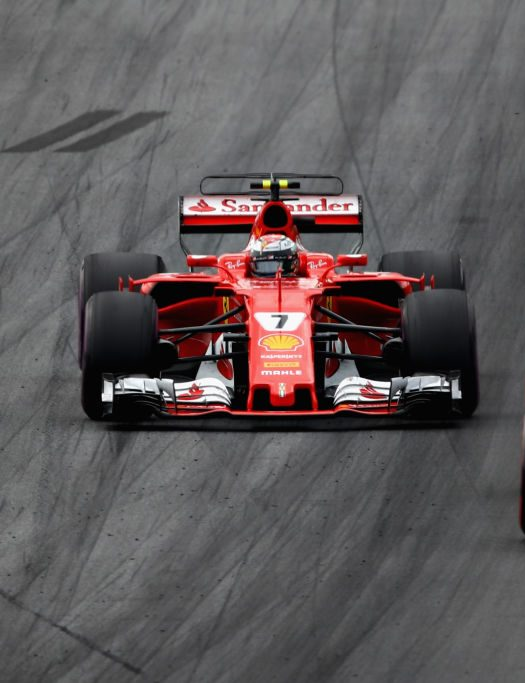
\includegraphics[width=0.8\textwidth]{Figures/F1.png}
\end{figure}
\tiny{I piloti di formula 1 hanno conoscenze superiori su come funziona un motore.}

\end{columns}
\end{frame}

\begin{frame}{5 principi basilari di questo corso (1)}
\phantomsection\label{principi-basilari-di-questo-corso-1}
\begin{enumerate}
\tightlist
\item
  la valutazione neuropsicologica forense è innanzitutto una valutazione
  clinica
\end{enumerate}

\vspace{3em}

\emph{Per una buona perizia/consulenza, bisogna avere competenze
cliniche (in particolare sono rilevanti le capacità diagnostiche)}
\end{frame}

\begin{frame}{5 principi basilari di questo corso (2)}
\phantomsection\label{principi-basilari-di-questo-corso-2}
\begin{enumerate}
\setcounter{enumi}{1}
\tightlist
\item
  In questo corso di Laurea (non solo nelle mie lezioni) il leitmotiv
  sarà che la valutazione forense hanno un ruolo fondamentale
  valutazioni di tipo cognitivo.
\end{enumerate}

\vspace{3em}

\emph{Un approccio che si sta imponendo in ambito forense è quello Di
sostanziare in maniera il più obiettiva/oggettiva possibile le vostre
argomentazioni.}

\emph{Questo si contrappone ad un approccio dominante alla valutazione
forense come semplice giudizio clinico, magari da fonte autorevole, o i
test proiettivi, etc.)}
\end{frame}

\begin{frame}{5 principi basilari di questo corso (3)}
\phantomsection\label{principi-basilari-di-questo-corso-3}
\begin{enumerate}
\setcounter{enumi}{2}
\tightlist
\item
  la valutazione neuropsicologica non è solo somministrazione di test ma
  raccolta di evidenze e stesura di una relazione.
\end{enumerate}

\vspace{3em}

\emph{Il concetto di raccolta di evidenze sarà un tema ricorrente di
questo scorso e gli aspetti statistici saranno presentati come alcune
delle possibili evidenze.}
\end{frame}

\begin{frame}{5 principi basilari di questo corso (4)}
\phantomsection\label{principi-basilari-di-questo-corso-4}
\begin{enumerate}
\setcounter{enumi}{3}
\tightlist
\item
  Rispetto alla valutazione neuropsicologica puramente clinica, nella
  valutazione forense ci sono possibili problemi aggiuntivi (es.
  simulazione). \vspace{3em}
\end{enumerate}

\emph{Non è richiesta solo competenza clinica, ma anche competenze
aggiuntive specifiche per valutazione forense.}
\end{frame}

\begin{frame}{5 principi basilari di questo corso (5)}
\phantomsection\label{principi-basilari-di-questo-corso-5}
\begin{enumerate}
\setcounter{enumi}{4}
\tightlist
\item
  In molti casi di forense (es. consulenze tecniche/perizie), a dispetto
  della valutazione neuropsicologica puramente clinica, è possibile che
  ci sia anche un' altra parte che farà un'altra valutazione e
  relazione, e l'obiettivo è anche creare una relazione più convincente
  (su basi argomentative e oggettive) dell'altra parte. \vspace{2em}
\end{enumerate}

\begin{figure}
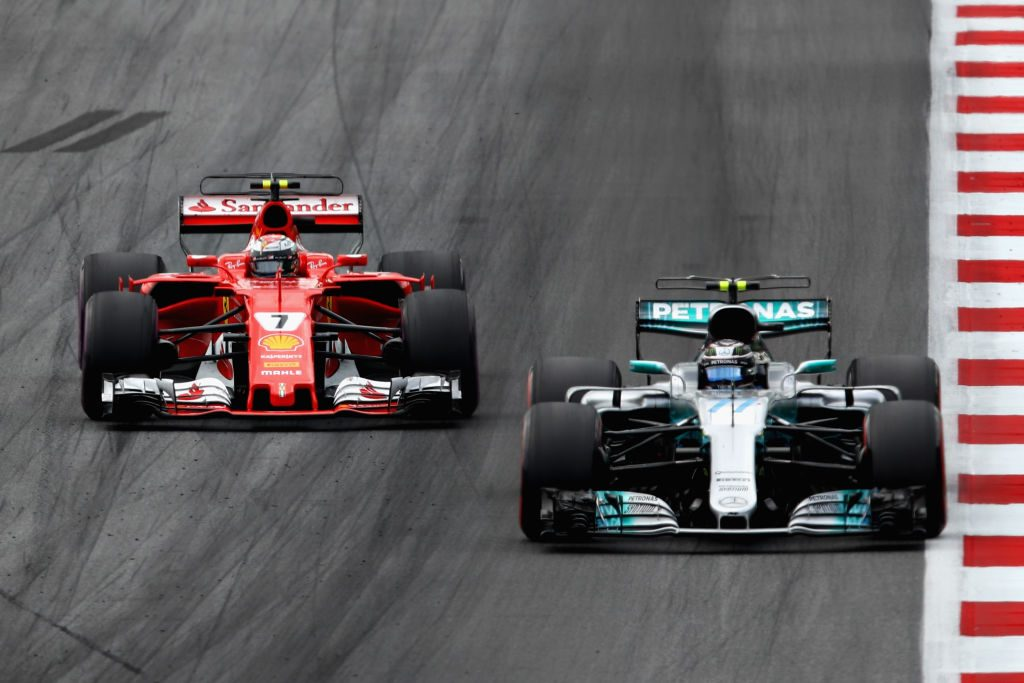
\includegraphics[width=0.4\textwidth]{Figures/F1_2.jpg}
\end{figure}
\end{frame}

\begin{frame}{Alcune domande a cui risponderete}
\phantomsection\label{alcune-domande-a-cui-risponderete}
\emph{Come posso dimostrare che I test utilizzati per la mia perizia
sono migliori di quelli dell'altra parte?}

\emph{Come posso dimostrare che nell'interpretare I test, l'altra parte
ha commesso un errore?}
\end{frame}

\begin{frame}{Focus sui test neuropsicologici}
\phantomsection\label{focus-sui-test-neuropsicologici}
Anche se la metodologia della valutazione neuropsicologica forense in
genere include vari aspetti, Il focus sulla lezione è sui test
neuropsicologici, su cosa sono, come si creano, come si interpretano i
risultati.

Questo perché l'utilizzo dei test rappresenta una fase fondamentale
della valutazione neuropsicologica.

\pause

(altre fasi che non sono trattate sono l'intervista, il colloquio con i
familiari, anche se sarà accennato il perché della loro rilevanza.)
\end{frame}

\begin{frame}{}
\phantomsection\label{section}
\emph{Perché si utilizzano i test in neuropsicologia clinica e in
neuropsicologia forense?}

\pause

Per ottenere informazioni rilevanti alla fine degli scopi della
valutazione e per superare i limiti di una valutazione soggettiva basata
solo su giudizi clinici.
\end{frame}

\begin{frame}{Perché non fornire direttamente la lista dei test
migliori?}
\phantomsection\label{perchuxe9-non-fornire-direttamente-la-lista-dei-test-migliori}
I test esistenti in neuropsicologia clinica sono innumervoli
(centinaia). Ogni elenco sarebbe parziale.

Il loro utilizzo dipende anche dalle circostanze e dalla domanda per cui
viene effettuata la valutazione.

I test moderni (e migliori) oggi, saranno potenzialmente superati l'anno
prossimo.
\end{frame}

\begin{frame}{Scegliere i test}
\phantomsection\label{scegliere-i-test}
\setlength{\fboxrule}{1mm}
\fcolorbox{red}{white}{\rule{0pt}{12pt}\hspace{2pt} Alcuni test sono meglio degli altri\hspace{2pt}}, ma la scelta dei test dipende anche  dalle circostanze: dal motivo della valutazione, dal contesto clinico, dalla patologia trattata, dal tempo a disposizione, dalle risorse economiche a disposizione, dai gusti del
neuropsicologo, etc.
\end{frame}

\begin{frame}{Perché sono importanti statistica e metodologia?}
\phantomsection\label{perchuxe9-sono-importanti-statistica-e-metodologia}
Non basta che un test sia ``pubblicato'' o ``validato'' perché sia
utilizzabile senza una riflessione critica.

\vspace{2em}

Grazie alle conoscenze metodologiche possiamo scegliere quale test è
meglio di un altro.

\pause
\vspace{2em}

\begin{center}
\begin{tikzpicture}[baseline=(current bounding box.center)]

% Prima riga: sbagliato - giusto
\node[anchor=west] at (0, 0) {\textbf{Sbagliato}};
\node[anchor=east] at (10, 0) {\textbf{Giusto}};
\draw[thick] (1.8, 0) -- (8.5, 0);

% X al centro
\node[text=red, font=\bfseries\Huge] at (5, 0) {X};

% Seconda riga: peggio - meglio
\node[anchor=west] at (0, -1.2) {\textbf{Peggio}};
\node[anchor=east] at (10, -1.2) {\textbf{Meglio}};
\draw[thick] (1.5, -1.2) -- (8.5, -1.2);

\end{tikzpicture}
\end{center}
\end{frame}

\begin{frame}{Perché psicometria/statistica a volte sono tralasciati?
(1/3)}
\phantomsection\label{perchuxe9-psicometriastatistica-a-volte-sono-tralasciati-13}
\begin{itemize}
\tightlist
\item
  Le abilità cliniche/forensi trascendono le conoscenze
  metodologiche/psicometriche. \emph{si può essere ottimi neuropsicologi
  clinici/forensi senza conoscere questi aspetti}
\end{itemize}
\end{frame}

\begin{frame}{Perché psicometria/statistica a volte sono tralasciati?
(2/3)}
\phantomsection\label{perchuxe9-psicometriastatistica-a-volte-sono-tralasciati-23}
\begin{itemize}
\tightlist
\item
  In neuropsicologia clinica non ci sono feedback chiari di un utilizzo
  inadeguato dei test.
\end{itemize}

\emph{(cosa succede se sbaglio clamorosamente nell'interpretazione di un
test? Non molto)}
\end{frame}

\begin{frame}{Perché psicometria/statistica a volte sono tralasciati?
(3/3)}
\phantomsection\label{perchuxe9-psicometriastatistica-a-volte-sono-tralasciati-33}
\begin{itemize}
\tightlist
\item
  È più facile fidarsi ``ciecamente'' di un test, e delegare la
  responsabilità al test (invece che prendersela come neuropsicologi) ed
  è più semplice considerarlo come uno strumento oggettivo.
\end{itemize}

\emph{(è stato il test a dirlo, non io!)}
\end{frame}

\begin{frame}{La situazione attuale}
\phantomsection\label{la-situazione-attuale}
In neuropsicologia forense non c'è (ad oggi) una forte cultura
psicometrica e statistica. Molti di questi limiti derivano direttamente
dalla neuropsicologia clinica.

Ci sono numerose pratiche problematiche (es. uso non consapevole dei
punti z
\end{frame}

\begin{frame}{L'Interpretative Approach}
\phantomsection\label{linterpretative-approach}
Anche se molto del materiale discusso proviene da testi di metodologia
generale, non ci sono (ancora) testi specifici di metodologia nella
neuropsicologia, tantomeno di forense.

L'approccio metodologico che descriverò in questa lezione, che abbiamo
chiamato ``Interpretative Approach'' permette rispondere in maniera
coerente a queste e a molte altre domande.

L'approccio che proponiamo mette al centro della valutazione
neuropsicologica la neuropsicologa/il neuropsicologo, non i test.
\end{frame}

\begin{frame}{L'Interpretative Approach e la neuropsicologia forense}
\phantomsection\label{linterpretative-approach-e-la-neuropsicologia-forense}
Per mettere al centro il neuropsicologo si parte da un approfondimento
di tutti quegli aspetti medotologici e statistici proprio per vedere fin
dove arrivano, dove si fermano e dove è che comincia realmente
l'intervento dello psicologo/neuropsicologo e la sua
\underline{interpretazione}.

Queste conoscenze vi aiuterannno non solo a conoscere meglio l'utlizzo
dei test, ma anche a capire bene tutte le altre evidenze che
raccoglierete per giungere ad un'interpretazione degli stessi (e a come
farlo attivamente), secondo basi statistiche.
\end{frame}

\begin{frame}{L'Interpretative Approach}
\phantomsection\label{linterpretative-approach-1}
Con la definizione dell'Interpretative approarch abbiamo cercato di
mettere ordine e più rigore a quella che è la regolare pratica clinica
in neuropsicologia (è applicabile alla pratica comune) e i più diffusi e
condivisi principi della psicometria applicati alla neuropsicologia

Attenzione: che ve ne rendiate conto o meno, comunque adotterete dei
principi nell'utilizzare i test.
\end{frame}

\begin{frame}{I 6 principi}
\phantomsection\label{i-6-principi}
L'interpretative approach si sviluppa a partire da 6 principi cardine

Molte delle spiegazioni saranno delle conseguenze logiche (o razionali)
a partire da questi principi cardine

Questi principi perlopiù cercando di esplicitare la common knowledge in
neuropsicologia clinica.
\end{frame}

\begin{frame}{Interpretative Approach - Principio 1}
\phantomsection\label{interpretative-approach---principio-1}
Il neuropsicologo svolge un ruolo attivo in ogni aspetto della
valutazione neuropsicologica.
\end{frame}

\begin{frame}{Interpretative Approach - Principio 2}
\phantomsection\label{interpretative-approach---principio-2}
La valutazione neuropsicologica è un processo razionale di raccolta di
informazioni sullo stato cognitivo di un soggetto esaminato e di
elaborazione di una conclusione.
\end{frame}

\begin{frame}{Interpretative Approach - Principio 3}
\phantomsection\label{interpretative-approach---principio-3}
In ogni valutazione neuropsicologica, il neuropsicologo deve integrare e
interpretare tutte le informazioni disponibili per trarre una
conclusione.
\end{frame}

\begin{frame}{Interpretative Approach - Principio 4}
\phantomsection\label{interpretative-approach---principio-4}
L'uso dei risultati dei test neuropsicologici implica sempre
un'interpretazione attiva da parte del neuropsicologo.
\end{frame}

\begin{frame}{Interpretative Approach - Principio 5}
\phantomsection\label{interpretative-approach---principio-5}
Il neuropsicologo deve essere consapevole delle inferenze implicite
quando interpreta le prove disponibili.
\end{frame}

\begin{frame}{Interpretative Approach - Principio 6}
\phantomsection\label{interpretative-approach---principio-6}
Una valutazione neuropsicologica può essere considerata tale solo quando
c'è stata un'osservazione diretta (di persona o a distanza) del
comportamento degli esaminati e un'\underline{interazione} diretta con
loro.
\end{frame}

\begin{frame}{Perchè è importante la consapevolezza dell'approccio?}
\phantomsection\label{perchuxe8-uxe8-importante-la-consapevolezza-dellapproccio}
Analogia con posizione filosofica

\begin{center}
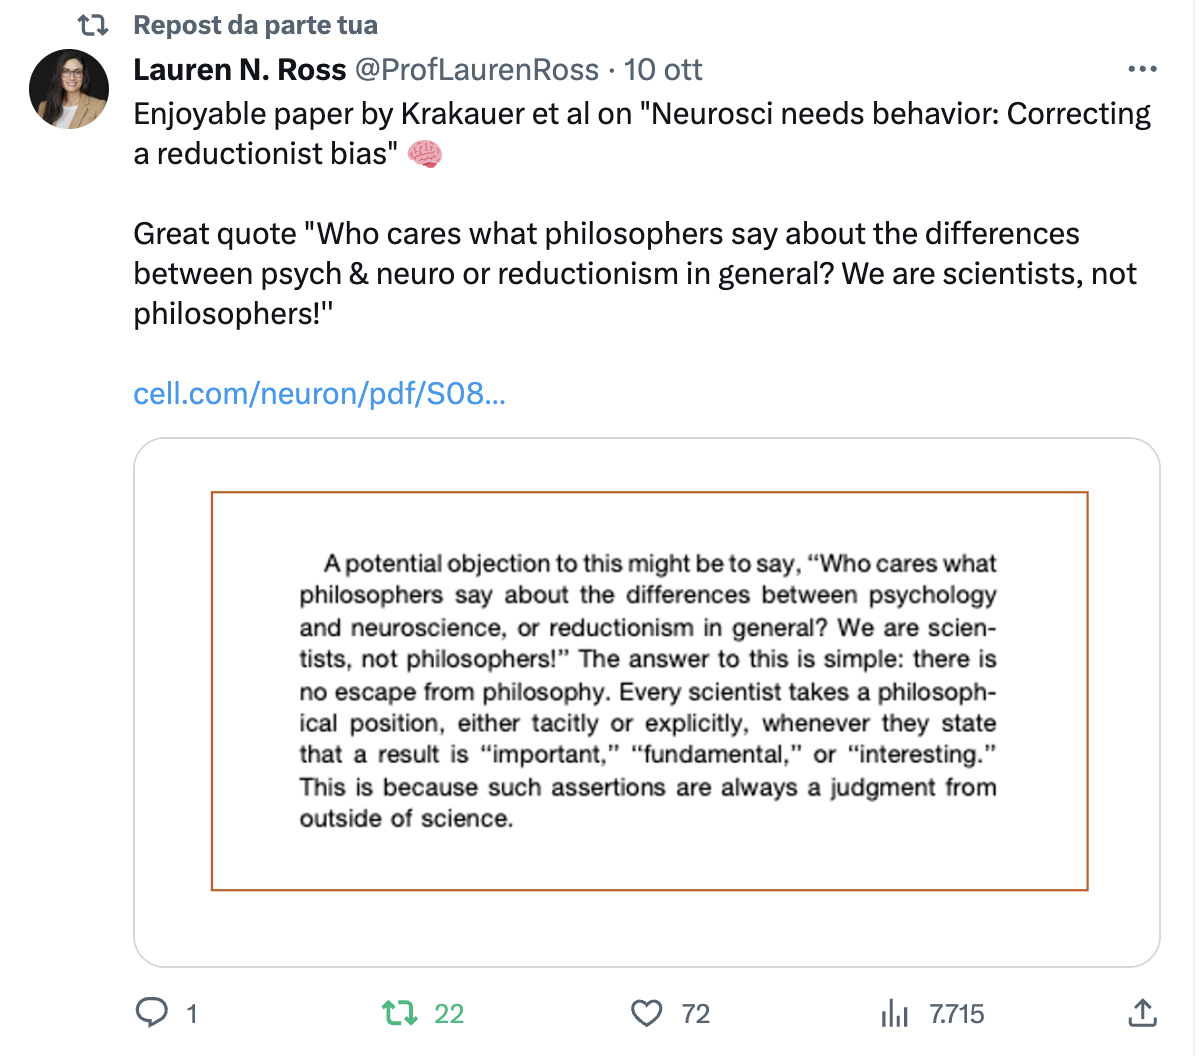
\includegraphics[width=\linewidth,height=0.7\textheight,keepaspectratio]{Figures/Ross_Twitter.png}
\end{center}
\end{frame}

\begin{frame}{L' ``Interpretative Approach'' alla neuropsicologia
clinica e forense}
\phantomsection\label{l-interpretative-approach-alla-neuropsicologia-clinica-e-forense}
A volte potrebbe sembrare che l'Interpretative approach ``giustifichi''
alcune arbitrarietà perchè deleghi inferenze e interpretazioni al
Neuropsicologo.

Questo è un errore. L'Interpretative approach, piuttosto, ha come
obiettivo far \emph{rendere consapevoli di una serie di intepretazioni}
da parte del Neuropsicologo, che comunque avvengono durante la
valutazione neuropsicologica e l'utilizzo dei test.

Conoscere quando queste avvengono porta ad una maggiore controllo di ci
che avviene nella valutazione e quindi a fare migliori valutazioni.
\end{frame}

\begin{frame}{L'Interpretative Approach alla neuropsicologia clinica e
forense}
\phantomsection\label{linterpretative-approach-alla-neuropsicologia-clinica-e-forense}
L'Interpretative approach nasce da esperienza di insegnamento di
neuropsicologia clinica (condiviso con Sara Mondini, Unipd e Marinella
Cappelletti, Goldsmiths London)

Spesso studentesse e studenti sono attratti dalla neuropsicologia
proprio per il rigore dei test rispetto, ad esempio, ad un semplice
colloquio o valutazione qualitativa. Questo può portare ad un' eccessiva
fiducia verso questi strumenti, oppure al dimenticarsi l'effettivo ruolo
più importante del neuropsicologo in vari aspetti del'utilizzo dei test.
\end{frame}

\begin{frame}{Valutazione neuropsicologica come raccolta di
informazioni}
\phantomsection\label{valutazione-neuropsicologica-come-raccolta-di-informazioni}
\pandocbounded{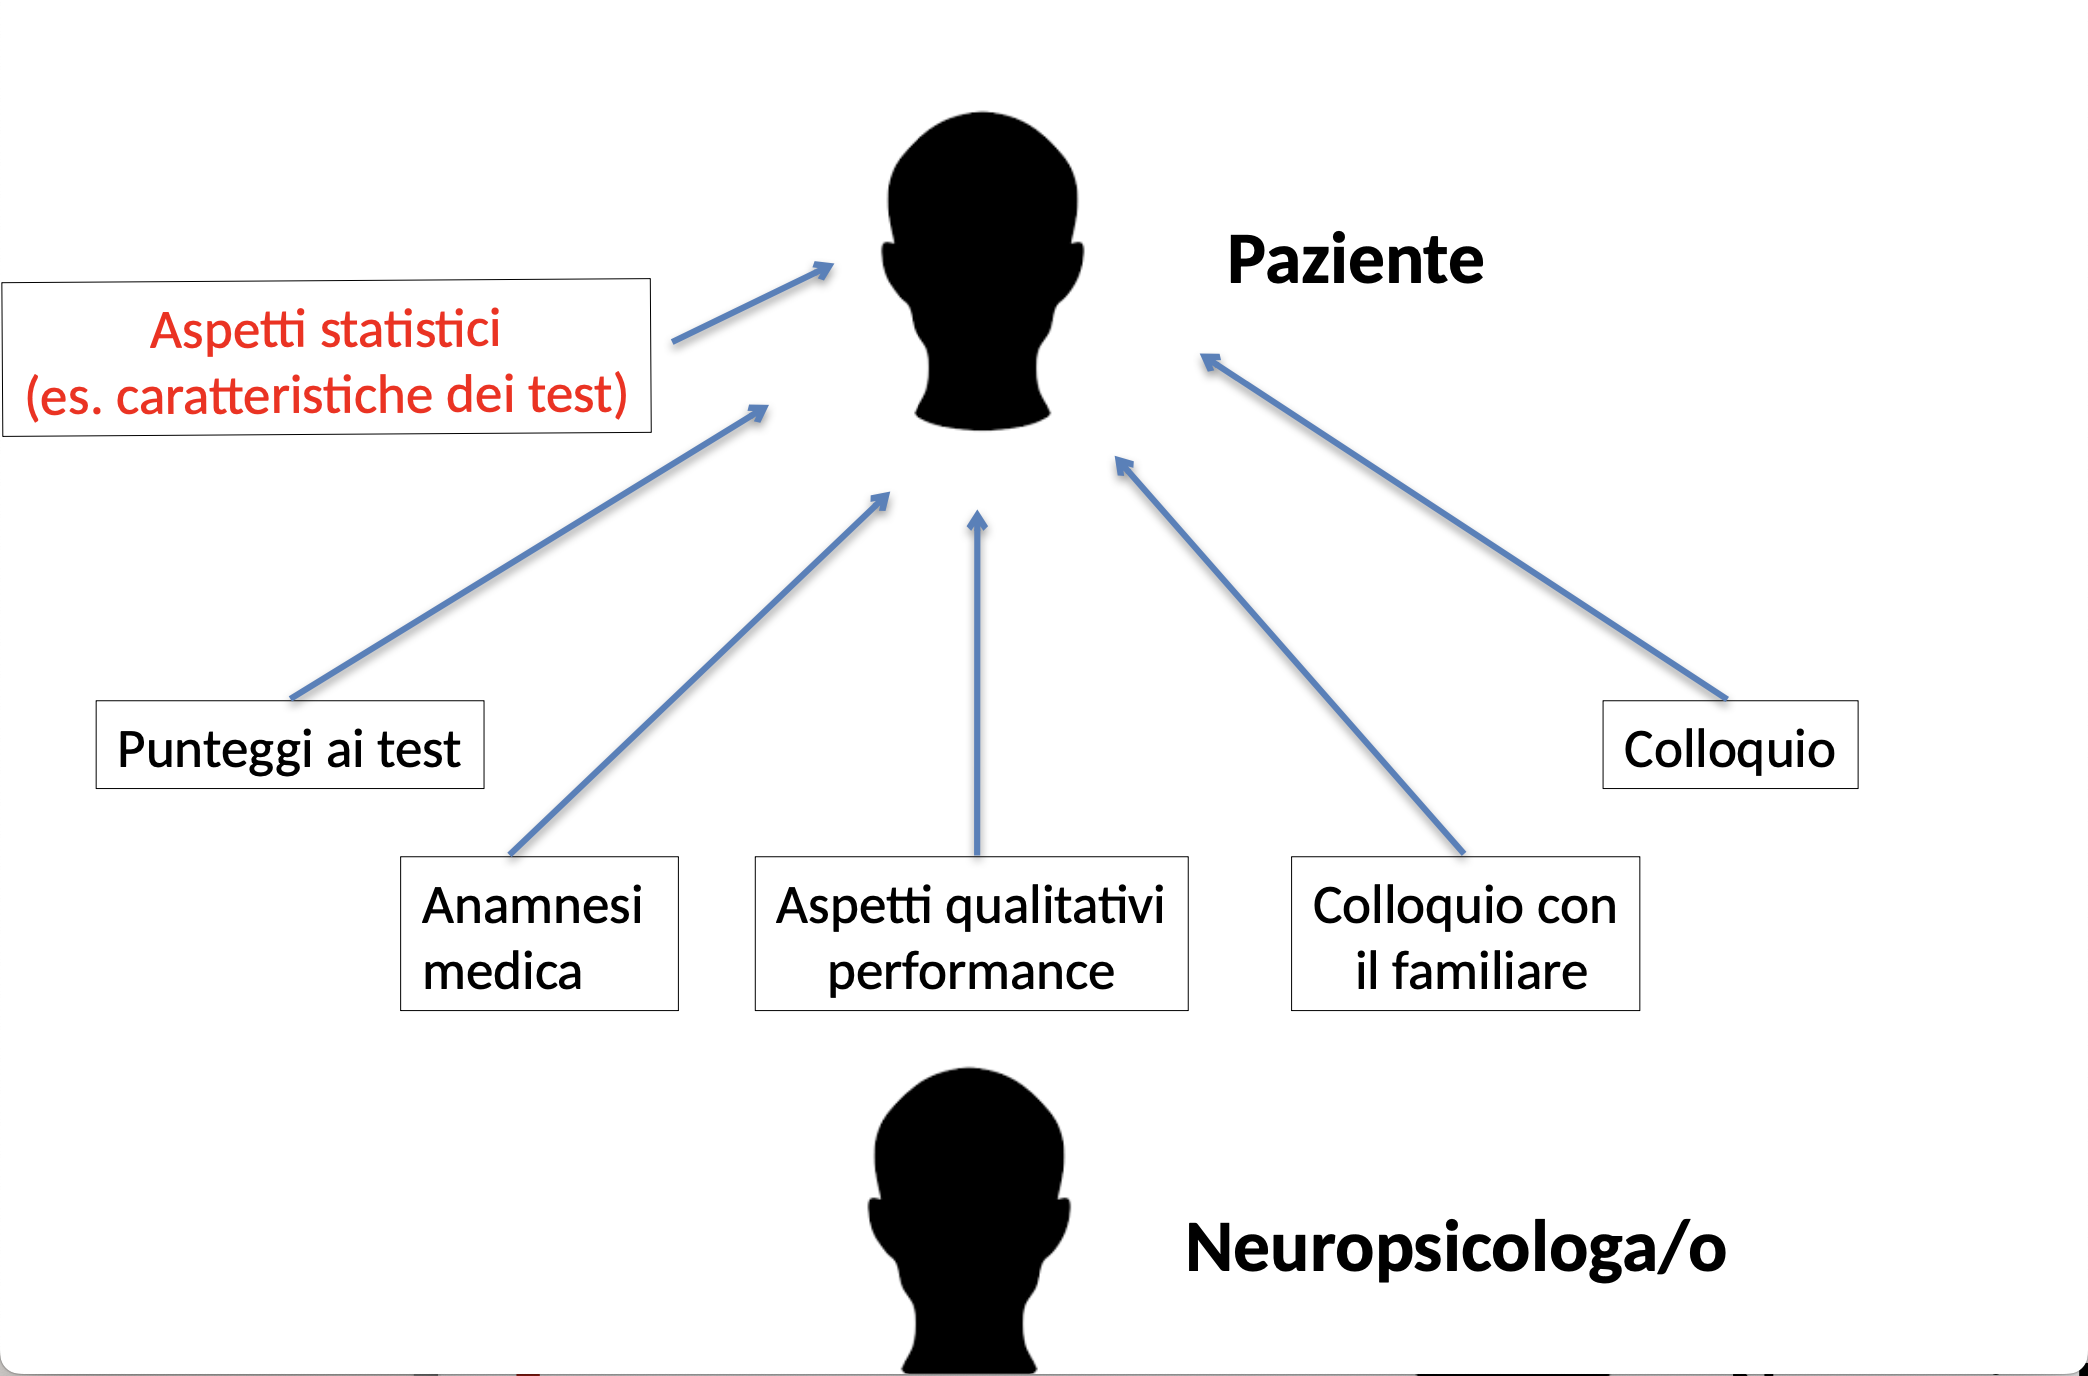
\includegraphics[keepaspectratio]{Figures/Active_collection.png}}
\end{frame}

\begin{frame}{Valutazione Neuropsicologica come raccolta di
informazioni}
\phantomsection\label{valutazione-neuropsicologica-come-raccolta-di-informazioni-1}
La raccolta di informazioni è un processo \textbf{attivo} del
neuropsicologo e dipende dalle sue conoscenze.

La stessa osservazione dipende dalle conoscenze, visto che I
comportamenti che notiamo o osserviamo \emph{(``teoreticità
dell'osservazione'')}

Così come tra queste conoscenze ci sono le conoscenze relative alle
caratteristiche dei test e alle informazioni che, realmente, possiamo
trarne.
\end{frame}

\begin{frame}{Valutazione neuropsicologica e forense}
\phantomsection\label{valutazione-neuropsicologica-e-forense}
Esistono vari obiettivi che potrebbe avere una valutazione forense,
alcuni dei quali molto complessi (es. giudicare la \emph{capacità di
intendere e volere}). In questo corso ci concentreremo su esempi sul
concetto di \textbf{danno}, ma anticipo che la definizione di danno è
diversa in ambito giuridico e in ambito clinico.
\end{frame}

\begin{frame}{Un esempio che ci accompagnerà}
\phantomsection\label{un-esempio-che-ci-accompagneruxe0}
\scriptsize

\emph{GH è un uomo di 68 anni, vedovo al centro di un contenzioso con
una compagnia di assicurazione.Al momento critico della nostra
valutazione ha appena avuto un trauma cranico in seguito ad un piccolo
incidente stradale, in cui però ha battuto la testa e perso conoscenza.
L'unico figlio sostiene che come conseguenza suo padre ha avuto un
importante peggioramento nel funzionamento cognitivo che si manifesta in
incapacità di comprendere bene ciò che gli viene detto.}

\emph{Nell'anamnesi di GH c'è però un evento rilevante. Quando era più
giovane (a 30 anni) sistemando il tetto di un garage, GH è caduto da una
scala e ha battuto la testa. Andato in ospedale non è stato
diagnosticato un trauma cranico, ma poco dopo sono accaduti una serie di
eventi: ha perso il lavoro che aveva da tempo in una piccola azienda e
ha divorziato con la moglie.}

\emph{La neuropsicologia forense entra in gioco per due motivi. I
consulenti per l'assicurazione sostengono che il problema di GH è legato
al trauma cranico subito molti anni prima e quindi non legato
all'incidente stradale. Secondo i consulenti incaricati da GH invece il
danno non è riconducibile al precedente (e non documentato) trauma, ma
solo a quello più recente.}
\end{frame}

\begin{frame}{Un esempio che ci accompagnerà (APACS)}
\phantomsection\label{un-esempio-che-ci-accompagneruxe0-apacs}
\begin{columns}
\column{0.5\textwidth}

\begin{figure}
\includegraphics[width=\textwidth]{Figures/APACS_test.png}
\end{figure}

\column{0.5\textwidth}
6 task: 2 per produzione e 4 per comprensione

\emph{(Arcara \& Bambini, 2016)}

3 punteggi globali

\end{columns}
\end{frame}

\begin{frame}{Un esempio che ci accompagnerà (Linguaggio Figurato 1)}
\phantomsection\label{un-esempio-che-ci-accompagneruxe0-linguaggio-figurato-1}
\pandocbounded{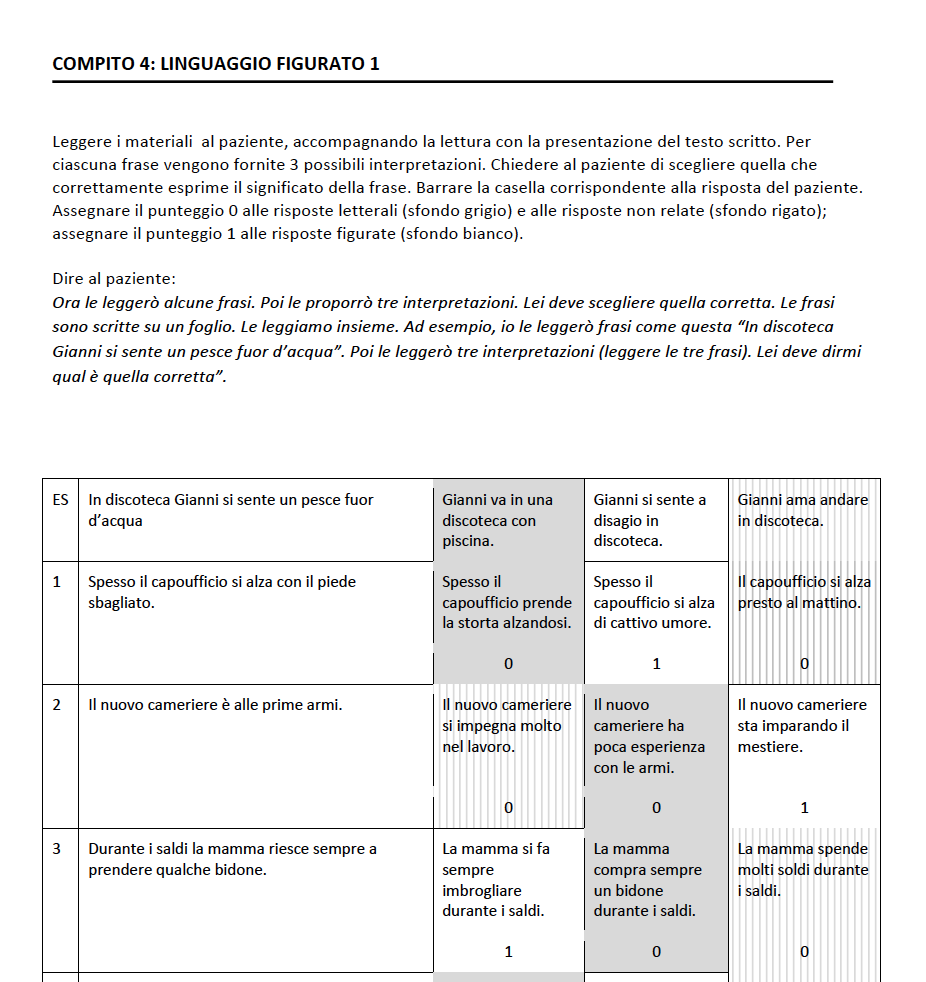
\includegraphics[keepaspectratio]{Figures/APACS_Fig_lang_1.png}}
\end{frame}




\end{document}
